\documentclass[a4paper, 14pt]{extarticle}
\usepackage{float}
% Поля
%--------------------------------------
\usepackage{geometry}
\geometry{a4paper,tmargin=2cm,bmargin=2cm,lmargin=3cm,rmargin=1cm}
%--------------------------------------


%Russian-specific packages
%--------------------------------------
\usepackage[T2A]{fontenc}
\usepackage[utf8]{inputenc}
\usepackage[english, main=russian]{babel}
%--------------------------------------

\usepackage{textcomp}

% Красная строка
%--------------------------------------
\usepackage{indentfirst}
%--------------------------------------


%Graphics
%--------------------------------------
\usepackage{graphicx}
\graphicspath{ {./images/} }
\usepackage{wrapfig}
%--------------------------------------

% Полуторный интервал
%--------------------------------------
\linespread{1.3}
%--------------------------------------

%Выравнивание и переносы
%--------------------------------------
% Избавляемся от переполнений
\sloppy
% Запрещаем разрыв страницы после первой строки абзаца
\clubpenalty=10000
% Запрещаем разрыв страницы после последней строки абзаца
\widowpenalty=10000
%--------------------------------------

%Списки
\usepackage{enumitem}

%Подписи
\usepackage{caption}

%Гиперссылки
\usepackage{hyperref}

\hypersetup {
	unicode=true
}

%Рисунки
%--------------------------------------
\DeclareCaptionLabelSeparator*{emdash}{~--- }
\captionsetup[figure]{labelsep=emdash,font=onehalfspacing,position=bottom}
%--------------------------------------

\usepackage{tempora}

%Листинги
%--------------------------------------
\usepackage{listings}
\lstset{
  basicstyle=\ttfamily\footnotesize,
  %basicstyle=\footnotesize\AnkaCoder,        % the size of the fonts that are used for the code
  breakatwhitespace=false,        % sets if automatic breaks shoulbd only happen at whitespace
  breaklines=true,                 % sets automatic line breaking
  captionpos=t,                    % sets the caption-position to bottom
  inputencoding=utf8,
  frame=single,                    % adds a frame around the code
  keepspaces=true,                 % keeps spaces in text, useful for keeping indentation of code (possibly needs columns=flexible)
  keywordstyle=\bf,       % keyword style
  numbers=left,                    % where to put the line-numbers; possible values are (none, left, right)
  numbersep=5pt,                   % how far the line-numbers are from the code
  xleftmargin=25pt,
  xrightmargin=25pt,
  showspaces=false,                % show spaces everywhere adding particular underscores; it overrides 'showstringspaces'
  showstringspaces=false,          % underline spaces within strings only
  showtabs=false,                  % show tabs within strings adding particular underscores
  stepnumber=1,                    % the step between two line-numbers. If it's 1, each line will be numbered
  tabsize=2,                       % sets default tabsize to 8 spaces
  title=\lstname                   % show the filename of files included with \lstinputlisting; also try caption instead of title
}
%--------------------------------------

%%% Математические пакеты %%%
%--------------------------------------
\usepackage{amsthm,amsfonts,amsmath,amssymb,amscd}  % Математические дополнения от AMS
\usepackage{mathtools}                              % Добавляет окружение multlined
\usepackage[perpage]{footmisc}
%--------------------------------------

%--------------------------------------
%			НАЧАЛО ДОКУМЕНТА
%--------------------------------------

\begin{document}

%--------------------------------------
%			ТИТУЛЬНЫЙ ЛИСТ
%--------------------------------------
\begin{titlepage}
\thispagestyle{empty}
\newpage


%Шапка титульного листа
%--------------------------------------
\vspace*{-60pt}
\hspace{-65pt}
\begin{minipage}{0.3\textwidth}
\hspace*{-20pt}\centering

\includegraphics[width=\textwidth]{emblem}
\end{minipage}
\begin{minipage}{0.67\textwidth}\small \textbf{
\vspace*{-0.7ex}
\hspace*{-6pt}\centerline{Министерство науки и высшего образования Российской Федерации}
\vspace*{-0.7ex}
\centerline{Федеральное государственное бюджетное образовательное учреждение }
\vspace*{-0.7ex}
\centerline{высшего образования}
\vspace*{-0.7ex}
\centerline{<<Московский государственный технический университет}
\vspace*{-0.7ex}
\centerline{имени Н.Э. Баумана}
\vspace*{-0.7ex}
\centerline{(национальный исследовательский университет)>>}
\vspace*{-0.7ex}
\centerline{(МГТУ им. Н.Э. Баумана)}}
\end{minipage}
%--------------------------------------

%Полосы
%--------------------------------------
\vspace{-25pt}
\hspace{-35pt}\rule{\textwidth}{2.3pt}

\vspace*{-20.3pt}
\hspace{-35pt}\rule{\textwidth}{0.4pt}
%--------------------------------------

\vspace{1.5ex}
\hspace{-35pt} \noindent \small ФАКУЛЬТЕТ\hspace{80pt} <<Информатика и системы управления>>

\vspace*{-16pt}
\hspace{47pt}\rule{0.83\textwidth}{0.4pt}

\vspace{0.5ex}
\hspace{-35pt} \noindent \small КАФЕДРА\hspace{50pt} <<Теоретическая информатика и компьютерные технологии>>

\vspace*{-16pt}
\hspace{30pt}\rule{0.866\textwidth}{0.4pt}

\vspace{11em}

\begin{center}
\Large {\bf Лабораторная работа № 1 } \\
\large {\bf по курсу <<Реализация однослойного перцептрона>>} \\
\large <<Теория искусственных нейронных сетей>>
\end{center}\normalsize

\vspace{8em}


\begin{flushright}
  {Студент группы ИУ9-71Б Баев Д.А \hspace*{15pt}\\
  \vspace{2ex}
  Преподаватель Каганов Ю. Т.\hspace*{15pt}}
\end{flushright}

\bigskip

\vfill


\begin{center}
\textsl{Москва 2023}
\end{center}
\end{titlepage}
%--------------------------------------
%		КОНЕЦ ТИТУЛЬНОГО ЛИСТА
%--------------------------------------

\renewcommand{\ttdefault}{pcr}

\setlength{\tabcolsep}{3pt}
\newpage
\setcounter{page}{2}

\section{Задание}\label{Sect::task}
1. Реализовать на языке высокого уровня однослойный персептрон и проверить его
работоспособность на примере искусственных данных типа цифр от 0 до 9 и букв
русского алфавита. Размер поля 5x4.

2. Исследовать работу персептрона на основе использования различных функций
активации. (Линейной, сигмоиды, гиперболического тангенса, ReLU).
\newpage
\section{Исходный код}

В рамках выполнения лабораторной работы были поставлены следующие цели:

1) Нужно осуществлять классификацию на 43 класса (33 буквы и 10 цифр).

2) Для этого будет реализовываться однослойный перцептрон с 43 нейронами: каждый нейрон отвечает за свой класс.

3) Эвристика подготовки датасета заключается в том, что метки изображений кодируются с помощью простейшего one-hot (это имеет значение в интерпретации результата).

4) В качестве функции потерь выбрана MSE, в качестве метрики выбрана точность.

Исходный код программы представлен в листингах~\ref{lst:code1}-~\ref{lst:code2}

\begin{figure}[H]
\begin{lstlisting}[language={},caption={Подготовка датасета},label={lst:code1}]
def create_image_array(text, font_path, image_size, font_size):
    image = Image.new('1', image_size, color='white')
    draw = ImageDraw.Draw(image)
    font = ImageFont.truetype(font_path, font_size)

    text_bbox = draw.textbbox((0, 0), text, font=font)
    text_width = text_bbox[2] - text_bbox[0]
    text_height = text_bbox[3] - text_bbox[1]

    x = (image_size[0] - text_width) / 2
    y = (image_size[1] - text_height) / 2

    draw.text((x, y), text, fill='black', font=font)

    image_array = np.array(image)
    return image_array



def generate_dataset(fonts_folder_train, fonts_folder_test, font_size):
    image_size = (5 * font_size, 4 * font_size)
    images_train = []
    images_test = []
    labels_train = []
    labels_test = []

    for char in alphabet:
        for font_file in os.listdir(fonts_folder_train):
            font_path = os.path.join(fonts_folder_train, font_file)
            if font_file.endswith(('.ttf', '.otf')):
                image_array = create_image_array(char, font_path, image_size, font_size)
                images_train.append(image_array)
                labels_train.append(classes_to_idx[char])


        for font_file in os.listdir(fonts_folder_test):
            font_path = os.path.join(fonts_folder_test, font_file)
            if font_file.endswith(('.ttf', '.otf')):
                image_array = create_image_array(char, font_path, image_size, font_size)
                images_test.append(image_array)
                labels_test.append(classes_to_idx[char])

    return images_train, images_test, labels_train, labels_test
\end{lstlisting}
\end{figure}


\begin{figure}[H]
\begin{lstlisting}[language={},caption={Реализация перцептрона},label={lst:code2}]
class Perceptron:
    def __init__(self, input_size, num_neurons, activation, activation_derivative):
        self.input_size = input_size
        self.activation = activation
        self.activation_derivative = activation_derivative
        self.weights = np.zeros(shape=(num_neurons, input_size + 1))

    def train(self, training_data, test_data, train_labels, test_labels, epochs, learning_rate):
        errors_train = []
        errors_test = []
        accuracy_train = []
        accuracy_test = []

        for j in range(epochs):
            running_error = 0
            run_acc = 0
            for i in range(len(training_data)):
                inputs = np.insert(training_data[i], 0, 1)
                label = train_labels[i]
                prediction = self.predict(inputs)
                error = prediction - label
                delta = error * self.activation_derivative(np.dot(self.weights, inputs))

                pred = np.argmax(prediction)
                if pred == np.argmax(label):
                    run_acc += 1
                running_error += MSE(prediction, label)

                self.weights -= learning_rate * np.outer(delta, inputs)
            running_error /= len(training_data)
            errors_train.append(running_error)
            accuracy_train.append(run_acc / len(training_data))

            running_error = 0
            run_acc = 0
            for i in range(len(test_data)):
                inputs = np.insert(test_data[i], 0, 1)
                label = test_labels[i]
                prediction = self.predict(inputs)

                pred  = np.argmax(prediction)
                if pred == np.argmax(label):
                    run_acc += 1
                running_error += MSE(prediction, label)

            running_error /= len(test_data)
            errors_test.append(running_error)
            accuracy_test.append(run_acc / len(test_data))

        return errors_train, errors_test, accuracy_train, accuracy_test

    def predict(self, inputs):
        summation = np.dot(self.weights, inputs)
        return self.activation(summation)
\end{lstlisting}
\end{figure}



\section{Результаты}

Результаты приведены на рисунках~\ref{fig:img1}-~\ref{fig:img8}

\begin{figure}[H]
\centering
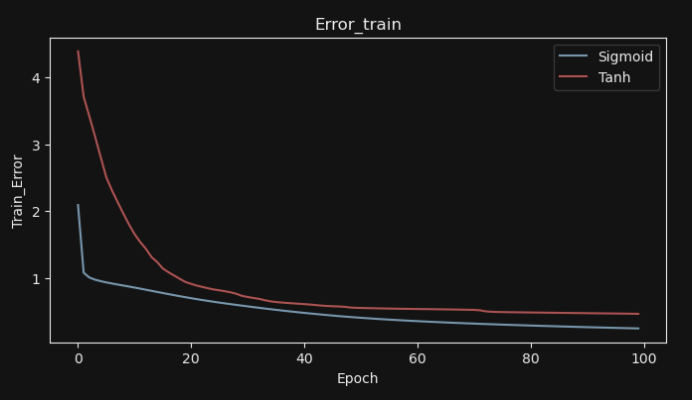
\includegraphics[width=0.8\textwidth]{images/res1.png}
\caption{График зависимости фунции потерь от количества эпох для сигмоиды и гиперболического тангенса на обучающей выборке}
\label{fig:img1}
\end{figure}


\begin{figure}[H]
\centering
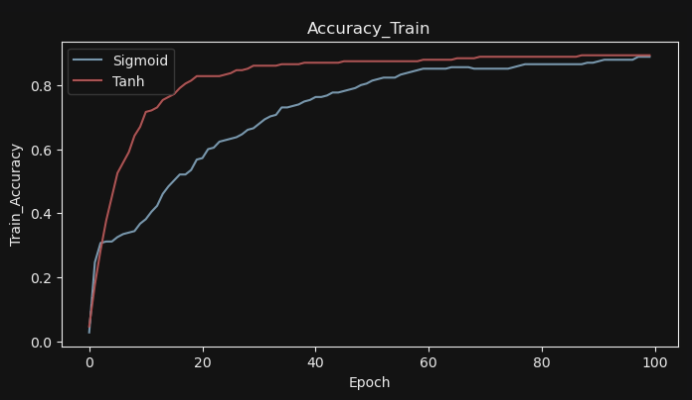
\includegraphics[width=0.8\textwidth]{images/res2.png}
\caption{График зависимости точности от количества эпох для сигмоиды и гиперболического тангенса на обучающей выборке}
\label{fig:img2}
\end{figure}


\begin{figure}[H]
\centering
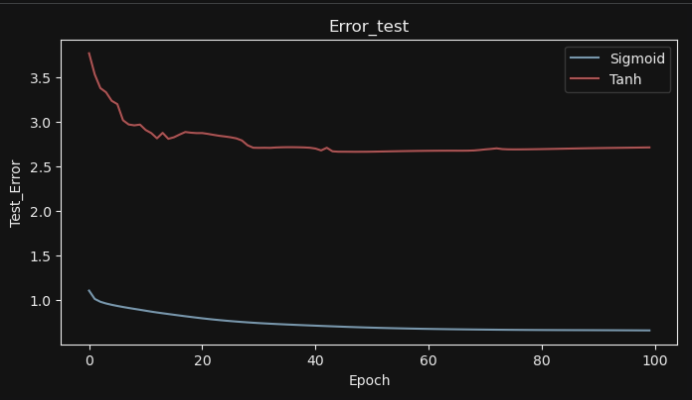
\includegraphics[width=0.8\textwidth]{images/res3.png}
\caption{График зависимости фунции потерь от количества эпох для сигмоиды и гиперболического тангенса на тестовой выборке}
\label{fig:img3}
\end{figure}


\begin{figure}[H]
\centering
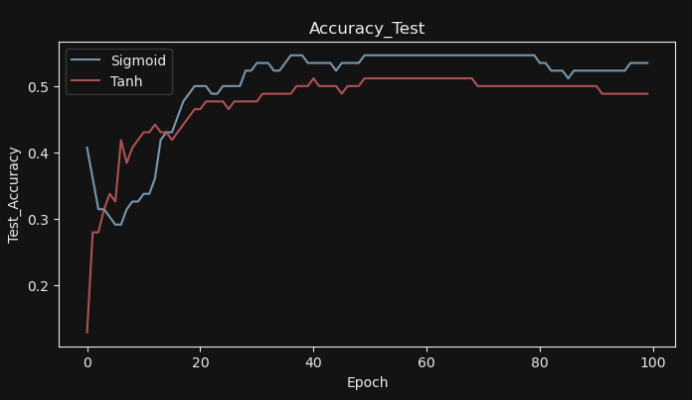
\includegraphics[width=0.8\textwidth]{images/res4.png}
\caption{График зависимости точности от количества эпох для сигмоиды и гиперболического тангенса на тестовой выборке}
\label{fig:img4}
\end{figure}


\begin{figure}[H]
\centering
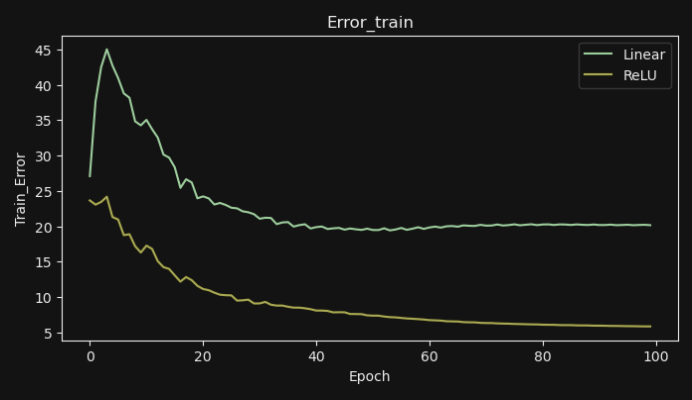
\includegraphics[width=0.8\textwidth]{images/res5.png}
\caption{График зависимости фунции потерь от количества эпох для линейной функции и ReLU на обучающей выборке}
\label{fig:img5}
\end{figure}


\begin{figure}[H]
\centering
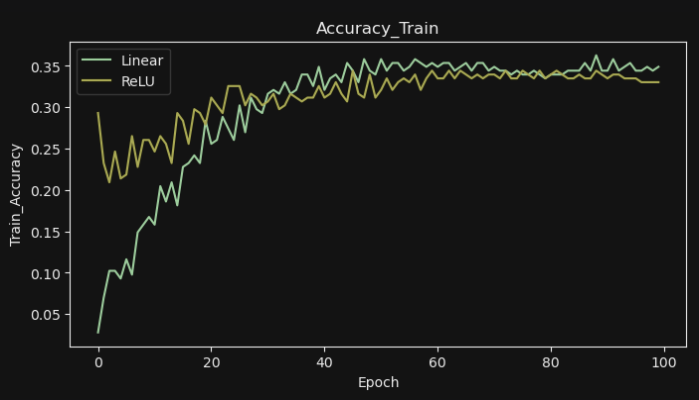
\includegraphics[width=0.8\textwidth]{images/res6.png}
\caption{График зависимости точности от количества эпох для линейной функции и ReLU на обучающей выборке}
\label{fig:img6}
\end{figure}


\begin{figure}[H]
\centering
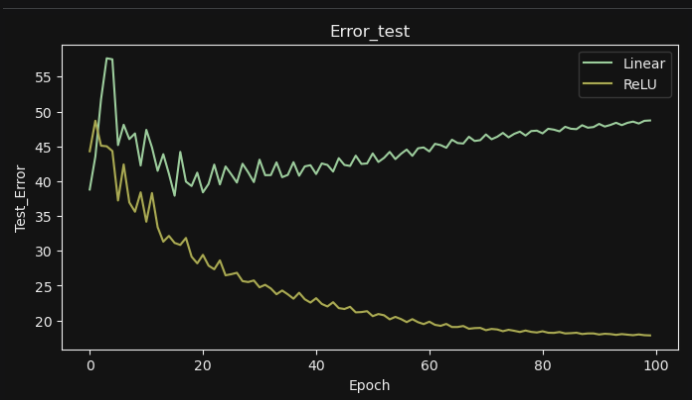
\includegraphics[width=0.8\textwidth]{images/res7.png}
\caption{График зависимости фунции потерь от количества эпох для линейной функции и ReLU на тестовой выборке}
\label{fig:img7}
\end{figure}


\begin{figure}[H]
\centering
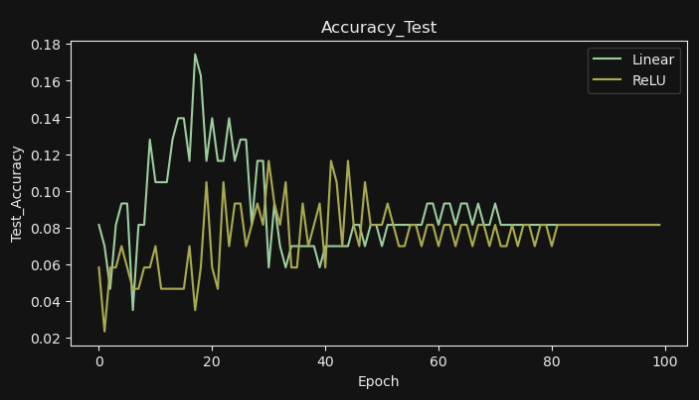
\includegraphics[width=0.8\textwidth]{images/res8.png}
\caption{График зависимости точности от количества эпох для линейной функции и ReLU на тестовой выборке}
\label{fig:img8}
\end{figure}

По графикам, видно, что при использовании сигмоиды и гиперболического тангенса, модель обучается успешно и показывает удолетворительный результат с учетом простоты своей архитектуры. Но для линейной функции и ReLU результат очень плох. Это связано с тем, что сигмоида и гиперболический тангенс являются ограниченными сверху и снизу, что имеет определяющее значение с учетом введеных эвристик.

\section{Выводы}
В рамках данной лабораторной работы был вручную реализован однослойный перцептрон, решающий задачу классификации. В процессе интерпретации результатов было установлено, что очень важно, какие именно эвристики вводятся на этапе постановки задачи и подготовки данных, так как это имеет решающее значение в построении архитектуры модели, даже самой простой.
\end{document}